%%%%%%%%%% NO OLVIDAR COLOCAR ESTE COMENTARIO CON EL NUMERO DE EJERCICIO %%%%%%%%%%%%%
%%%%%%%%%%%%%%%%%%% EJERCICIO 1 %%%%%%
%%Text bf para negrilla , el \\ es para el salto de linea.
%%El primer \\ hace un espacio en el texto y el 2 \\ crea otro espacio

\textbf{Ejemplo 1}\newline
Una persona compra un terreno cuyo valor al contado es de 2.000.000 COP. Si le dan la facilidad para pagarlo en cuatro periodos trimestre vencidos del mismo valor cada uno y, además se le cargará un interés del 40\% nominal anual trimestre vencido, hallar el valor de la cuota trimestral de amortización.\\ \\

\textbf{Solución.}\\
\begin{center}

	\renewcommand{\arraystretch}{1.5}% Margenes de las celdas
	%Creación de la cuadricula
	\begin{longtable}{|C{0.3\linewidth}|C{0.3\linewidth}|C{0.3\linewidth}| }
		%Creamos una linea horizontal
		\hline
		%Definimos el color de la primera fila
		\rowcolor[HTML]{FFB183}
		%%%%% INICIO ASIGNACIÓN FECHA FOCAL %%%%%%%
		%%%%%%%%%% INICIO TITULO
		%Lo que se hace aquí es mezclar las 3 columnas en una sola
		\multicolumn{3}{|c|}{\cellcolor[HTML]{FFB183}\textbf{1. Asignación período focal}}   \\ \hline
		%%%%%%%%%% FIN TITULO
		%%%%% INICIO DECLARACIÓN DE VARIABLES %%%%%%%
		\multicolumn{3}{|c|}{$pf : 0 ptv$} \\ \hline
		%Definimos el color de la primera fila
		\rowcolor[HTML]{FFB183}
		%%%%% INICIO DECLARACIÓN DE VARIABLES %%%%%%%
		%%%%%%%%%% INICIO TITULO
		\multicolumn{3}{|c|}{\cellcolor[HTML]{FFB183}\textbf{2. Declaración de variables}}                                                                                   \\ \hline
		%%%%%%%%%% FIN TITULO
		%%%%%%%%%% INICIO DE MATEMÁTICAS
		\multicolumn{1}{|c|}{\cellcolor[HTML]{FFB183}\textbf{Valores monetarios}}    & \multicolumn{1}{c|}{\cellcolor[HTML]{FFB183}\textbf{Valores no monetarios}} & \multicolumn{1}{c|}{\cellcolor[HTML]{FFB183}\textbf{Incógnitas}} \\ \hline
		VP = 2.000.000 COP & $j_ {1} = 40\% \textit{ natv} \equiv 10\% \textit{ptv} = i_1$ & $ R = { ? } COP $ \\
		& $n_{1}= 1 \textit{ ptv}$ & \\
		& $n_{2}= 2 \textit{ ptv}$ & \\
		& $n_{3}= 3 \textit{ ptv}$ & \\
		& $n_{4}= 4 \textit{ ptv}$ & \\ \hline
		%%%%%%%%%% FIN DE MATEMÁTICAS
		%%%%% FIN DECLARACIÓN DE VARIABLES


		%%%%% INICIO FLUJO DE CAJA
		\rowcolor[HTML]{FFB183}
		\multicolumn{3}{|c|}{\cellcolor[HTML]{FFB183}\textbf{3. Diagrama de flujo de caja}}                                                                                  \\ \hline
		%Mezclamos 3 columnas y pondremos el dibujo
		%%%%%%%%%%%%% INSERCIÓN DE LA IMAGEN
		\multicolumn{3}{|c|}{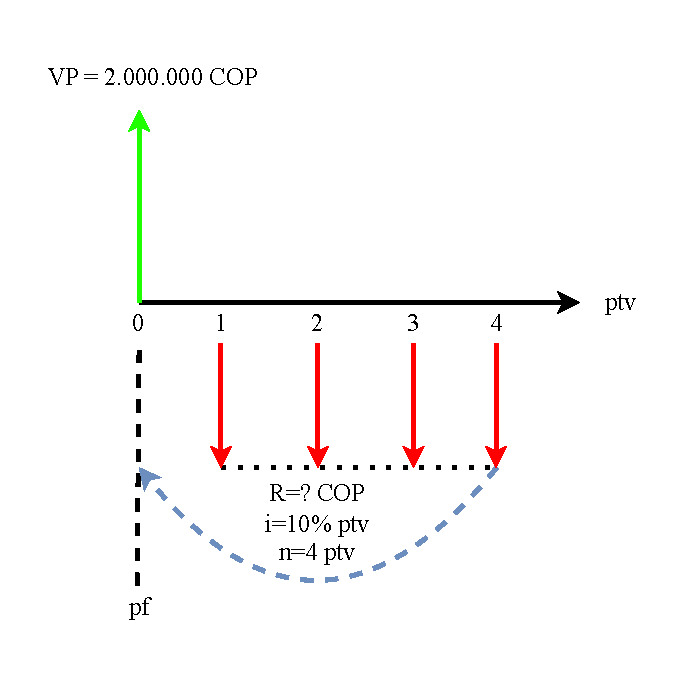
\includegraphics[trim=-5 -5 -5 -5, scale=0.8]{4_Capitulo/img/ejemplos/1/Exportados/Graficas Latex - Ejemplo 1.pdf} }                                   \\ \hline
		%%%%%%%%%%%%% FIN INSERCIÓN DE IMAGEN

		%%%%%FIN FLUJO DE CAJA



		%%%%% INICIO DECLARACIÓN FORMULAS
		%%%%%%%%%%% INICIO TITULO
		\rowcolor[HTML]{FFB183}
		\multicolumn{3}{|c|}{\cellcolor[HTML]{FFB183}\textbf{4. Declaración de fórmulas}}                                                                                    \\ \hline
		%%%%%%%%%%% FIN TITULO
		%%%%%%%%%%% INICIO MATEMÁTICAS
		\multicolumn{3}{|c|} {$VP=R\frac{1-(1+i)^{-n}}{i}$ Valor presente serie uniforme vencida}   \\
		\multicolumn{3}{|c|} {$P=F(1+i)^{-n}$ Valor presente}   \\ \hline
		%%%%%%%%%% FIN MATEMÁTICAS
		%%%%%% INICIO DESARROLLO MATEMÁTICO
		\rowcolor[HTML]{FFB183}
		%%%%%%%%%%INICIO TITULO
		\multicolumn{3}{|c|}{\cellcolor[HTML]{FFB183}\textbf{5. Desarrollo matemático}}                                                                                      \\ \hline
		%%%%%%%%%% FIN TITULO
		%%%%%%%%%% INICIO MATEMÁTICAS
		%%% - DESARROLLO MEDIANTE VALOR PRESENTE -
		\multicolumn{3}{|c|}{\cellcolor[HTML]{FFB183}\textbf{Resolviendo el problema utilizando la fórmula de valor presente}}\\ \hline
		\multicolumn{3}{|c|}{ P = 2.000.000 \ $n = 1, 2, 3, 4$ \quad } \\
		\multicolumn{3}{|c|}{  2.000.000 COP =$ R(1 + 0,1)^{−1} + R(1 + 0,1)^{−2}+R(1+0,1)^{−3} + R(1+0,1)^{−4}$}\\
		\multicolumn{3}{|c|}{  2.000.000 COP =$ R[(1+0,1)^{−1} + (1+0,1)^{−2} + (1+0,1)^{−3}+ (1 + 0, 1) ^{−4} ]$} \\
		\multicolumn{3}{|c|}{  2.000.000 COP =$ R(3,169865)$}\\
		\multicolumn{3}{|c|}{ R = 2.000.000 COP / 3,169865}\\
		\multicolumn{3}{|c|}{ R = 630.942 COP}\\ \hline
		%%%%%%%%%% DE FORMA RESOLVIENDO MEDIANTE VALOR PRESENTE SERIE UNIFORME
		\multicolumn{3}{|c|}{\cellcolor[HTML]{FFB183}\textbf{Resolviendo el problema utilizando la fórmula de valor presente serie uniforme}}\\ \hline
		\multicolumn{3}{|c|}{ VP = 2.000.000 \ $n =4$ \ $i =0.1 $ \quad} \\
		\multicolumn{3}{|c|}{ 2.000.000 COP= $ R\frac{1-(1+0.1)^{-4}}{0.1} $}\\
		\multicolumn{3}{|c|}{ 2.000.000 COP= $ R(3,16987) $}\\
		\multicolumn{3}{|c|}{ R= $ \frac{2.000.000 COP}{3,16987} $}\\
		\multicolumn{3}{|c|}{ R=  630.942 COP }\\ \hline
		%%%%%% FIN DESARROLLO MATEMÁTICO

		\rowcolor[HTML]{FFB183}
		\multicolumn{3}{|c|}{\cellcolor[HTML]{FFB183}\textbf{6. Respuesta}}    \\ \hline

		\multicolumn{3}{|c|}{ El valor de la cuota trimestral de amortización es de 630.942 COP } \\ \hline
	\end{longtable}
	%Se crean dos lineas en blanco para que no quede el siguiente texto tan pegado
	%\newline \newline
\end{center}
%%%%%%%%%%%%%%%%%%%%%%%%%%FIN EJERCICIO X %%%%%%%%%%%%%%%%%%%%%%%%%%%
